\documentclass{article}
\usepackage[auth-sc-lg]{authblk}
\usepackage{booktabs}
\usepackage{subcaption}
\usepackage{pgfplots}
\usepackage{hyperref}
\usepackage{amsmath}
\usepackage{setspace}
\usepackage{graphicx}
\usepackage{comment}

\definecolor{DeepBlue}{HTML}{0098E9}
\definecolor{DeepRed}{HTML}{FF297F}
\definecolor{DeepGreen}{HTML}{12B819}
\pgfplotsset{
  compat=1.12,
  deeploss/.style={
    width=0.9\textwidth,
    height=3in,
    x tick label style={font=\footnotesize},
    y tick label style={font=\footnotesize},
    axis x line*=bottom,
    xmajorgrids=true,
    ymajorgrids=true,
    major grid style={dotted},
    xlabel={Epoch},
    ylabel={\textcolor{DeepRed}{Validation loss}},
    axis y line*=right,
    ymin=-0.1,
    ymax=2.1
  },
  deepaccuracy/.style={
    width=0.9\textwidth,
    height=3in,
    axis x line=none,
    y tick label style={font=\footnotesize},
    ylabel={\textcolor{DeepBlue}{Validation accuracy (\%)}},
    axis y line*=left,
    ymin=-5,
    ymax=105
  }
}

\newcommand{\dataset}[1]{\textsf{#1}}


\title{Image Anomaly Detection with Neural Networks}
\author[1]{Ross Churchley}
\author[2]{Omeiza Olumoye}
\author[3]{Pawan Patel}
\author[4]{Jonathan Smith}
\author[5]{Parker Williams}
\author[3]{Ruiyu Yang}
\author[6]{Jesse Berwald}
\author[6]{Janet Keel}
\affil[1]{Simon Fraser University}
\affil[2]{University of Texas}
\affil[3]{Indiana University}
\affil[4]{Acadia University}
\affil[5]{University of California}
\affil[6]{Target Corporation}


\begin{document}
\maketitle
\onehalfspace
\section{Introduction}
  Neural networks are a statistical learning paradigm inspired by the structure of the neurons in the human brain.  The brain learns by forming and strengthening connections between neurons when exposed to various stimuli. Analogously, neural networks ``learn'' by adjusting connecting maps between computational layers when exposed to data according to some objective function.

  Interest in neural networks has periodically waxed and waned since the development of the backpropagation algorithm in the mid-1970s~\cite{werbos}. Recently, computational improvements have caused a resurgence in neural networks: modern GPU processing is now highly optimized for 2-dimensional convolution, allowing for much deeper networks. Architectural developments have also driven success in this field; competitions have seen dramatic new records set for accuracy and speed using algorithms that are less complex than the previous record holders. New and notable results include~\cite{INC,RFH}. GoogleNet has also enjoyed recent success~\cite{GDWC} using networks inspired by models for the visual cortex, and their creation of a special ``inception layer'' is similar to the network-in-network approach by Lin et al.~\cite{NIN}.

  Many open questions and technical challenges still surround convolutional neural networks. It is often unclear what situations a new technique or structure will apply to and the circumstances under which it will fail.   Still, the current approaches suggest that as-yet-undiscovered techniques could lead to sparser, more accurate networks. Known theoretical bounds have been documented by Arora et al.~\cite{PB}.


\section{Convolutional Neural Networks}

  A \emph{convolutional neural network (CNN)} is a sequence of computational layers, each ``feeding forward'' into the next. Throughout this section, we will assume the input for a network is an $n\times n$ array representing an image. A layer can be of several different types:

  \begin{itemize}
    \item A \emph{convolution layer} applies $m$ different $k\times k$ learned convolution kernels to the image, producing a group of $m$ $(n-k+1) \times (n-k+1)$ images. Over the course of the learning process, the kernels in the first convolution layer will typically specialize to extract low-level features like edges or corners of an image (see Figure~\ref{kernels}). Deeper convolution layers will recognize patterns of these features in order to extract higher-level features.

    \item A \emph{max-pooling layer} is a deterministic step that reduces the dimension of an image by a factor of $k$. It simply divides an input image into $k \times k$ sub-blocks and takes the maximal pixel value in each block.

    \item A \emph{fully-connected layer} discards the positional information of the input image and treats it as an $n^2$-dimensional vector $x$. It then applies a learned affine transformation $Wx + b$ to aggregate information from the individual feature maps discovered by the convolutional layers.
  \end{itemize}

  \begin{figure}[ht]
    \centering
    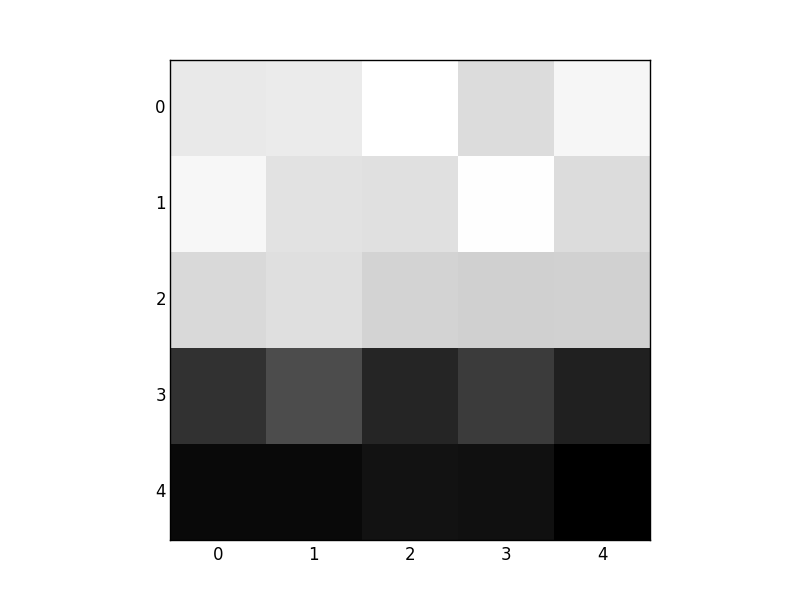
\includegraphics[scale=0.25]{img/Solid0-4.png}
    \caption{A $5\times 5$ convolution kernel which has learned to detect thick edges.}\label{kernels}
  \end{figure}

  Networks typically end with at least one fully connected layer, with the output dimension set to the number of categories one wishes to divide the images into.

  After each layer, an activation function is called. This corresponds biologically to the activation potential of a neuron firing, but also serves a purpose of rescaling the data layer to layer. As we will see, the choice of activation function can be vital and should be made within the context of the data.

  Today, the most popular activation function for deep neural networks is the \emph{rectifier} or \emph{rectified linear unit (ReLU)}~\cite{lecun2015}
  \[ f(x) = \max \{0, x\}. \]
  In this paper, we also consider the so-called \emph{leaky rectifier}~\cite{leakyrectify}
  \[ f(x) = \begin{cases} x & x \geq 0 \\ 0.01 x & x < 0. \end{cases}. \]
  Other activations that can be found in the literature include $\tanh(x)$ and the sigmoid function ${(1+e^{-x})}^{-1}$.
  The \emph{softmax} activation function
  \[ {\phi(x)}_j=\frac{e^{x_j}}{\sum_{k=1}^K e^{x_k}} \]
  is often added to the fully-connected layer at the end of the network, so that its output can be interpreted as the network's confidence, expressed as a probability, that the image falls into the $j$th category

  To make the network ``learn'', one must specify an objective function for it to minimize. In this report, we use the \emph{cross-entropy} function
  \[ L = - t \log(p) - (1-t) \log(1-p), \]
  where $p, (1-p)$ is the output of the network and $t, (1-t)\in \{0,1\}$ indicate the ``true distribution''.

  The learning process uses a backpropagation algorithm to adjust the parameters given a labeled training dataset. Layer by layer, the gradient of the objective function $L$ is computed with respect to the learned parameters $W$ at that layer, and the parameters are adjusted in that direction, i.e.
  \[ W_{i+1}=W_i-\epsilon\nabla L(W_i) \]
  where $\epsilon$ is a fixed number called the \emph{learning rate} chosen in advance. Choosing $\epsilon$ for a particular dataset and network is also an art, and can qualitatively change the learning progress.


\section{Anomalous images}

  Retailers currently manage very large numbers of digital photographs, typically within a very narrow scope. Nearly all images are subject to some form of image manipulation, and because of the sheer number of images, some errors are inevitable. Leveraging the focused nature of the data (photos of similar objects, already categorized) it is hoped that it may be feasible for a convolutional neural network to learn to detect anomalous images.

  Image manipulation errors, however, may come in many forms. Some high-profile cases have three models with seven hands between them due to bad photo compositing; more commonly, overzealous smudging, erasing, or stretching leads to models with bizarre proportions, artificial smoothness, or missing parts.

  Given the wide range of potential anomalies --- and lack of a labeled set of ``anomalous'' pictures at the scale we need for neural network training --- we need to focus on a particular type of error which is easily reproduced programmatically. In this report, we consider the problem of detecting white rectangles added to an image, simulating the type of error where portions of an image are damaged or deleted.


\section{Methodology}

  We built several convolutional neural networks using the Lasagne Python library~\cite{lasagne}, which is built on top of Theano~\cite{theano1,theano2}. Each network was trained up to four datasets using the GPU architecture on the Minnesota Supercomputing Institute's Mesabi compute cluster. The four datasets used in this paper are as follows:

  \begin{itemize}
    \item \dataset{Binary} (10000 images). Solid black backgrounds.
    \item \dataset{Solid} (10000 images). Solid backgrounds of varying brightnesses.
    \item \dataset{Flickr} (30000 images). Photos from Flickr, chosen from several of the most popular tags (e.g.\ ``canon'', ``nikon'', ``travel'').
    \item \dataset{Target} (131784 images). Target's complete catalogue of product images, each consisting of a product and/or model against a white background.
  \end{itemize}

  \begin{figure}
    \centering
      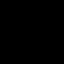
\includegraphics{img/black}\quad
      
\includegraphics{img/solid}\quad
      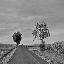
\includegraphics{img/flickr}\quad
      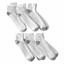
\includegraphics{img/target}\bigskip

      
\includegraphics{img/black+rect}\quad
      
\includegraphics{img/solid+rect}\quad
      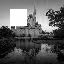
\includegraphics{img/flickr+rect}\quad
      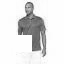
\includegraphics{img/target+rect}
      \caption{Examples of images from the \dataset{Binary}, \dataset{Solid}, \dataset{Flickr}, and \dataset{Target} datasets}
  \end{figure}

  Each image was resized to $64\times 64$ pixels and converted to greyscale. To each image, a white $16\times 16$ square was added with probability $\frac{1}{2}$ in a position chosen uniformly at random (among positions having the square entirely inside the image). The resulting greyscale image was then read in as a $64\times 64$ array and normalized so each pixel took values in $[0, 1]$.

  Each dataset was split into three parts: a \emph{training set} (80\% of the images) was used for network training; a \emph{validation set} (10\%) used to measure the performance of the network during the training process; and a \emph{test set} (10\%) used to measure the performance of the network after it has finished learning. In Section~\ref{results}, we report for each network the average value of the objective function on the test set (the \emph{test loss}) and the proportion of images in the test set correctly identified by the network (the \emph{test accuracy}).

  The learning process for each network and dataset was run for 100 \emph{epochs} (full passes through the training set) using the Nesterov momentum update scheme with a learning rate of 0.001 and momentum of 0.9. In Section~\ref{charts} we plot for each network the loss and accuracy on the validation set at each epoch in the learning process.


\section{Comparison of network architectures}\label{results}
  \subsection{Logistic regression}

    The most basic neural network is the logistic regression, consisting of a single fully-connected layer with the softmax activation function.

    \begin{table}[ht]
      \centering
      \begin{tabular}{lrr}\toprule
        \textbf{Dataset} & \textbf{Test Loss} & \textbf{Accuracy (\%)}\\\midrule
        \dataset{Binary} & 0.0007 & 100.0\% \\
        \dataset{Solid}  & 0.8464 &  74.9\% \\ % d02787bd-1a75-4e60-b526-e314f2fe25b7
        \dataset{Flickr} & 1.0338 &  55.0\% \\ % d69afb60-d39c-405c-b80a-4dae431c1f86
        \dataset{Target} &    --- &     --- \\ \bottomrule
      \end{tabular}
    \end{table}

    As a simple and standard model, linear regression is a useful baseline to compare our convolutional networks with. It does well on the \dataset{\dataset{Binary}} dataset, as one might expect: applying a roughly-uniform $W$ is similar to computing the average brightness of pixels in the image, from which the presence or absence of a white square on a black background can easily be determined. But this strategy does not fare as well when the brightness of the background can vary, as it does in the \dataset{Solid} dataset. And on the noisy \dataset{Flickr} dataset, this simple model is not much better than random.

    Although logistic regression outperforms coin-flipping, the training process does not produce significantly better results than a randomly-initialized $W$ (see Figures~\ref{logistic-binary},~\ref{logistic-solid}, and~\ref{logistic-flickr}) In fact, single-layer networks are inherently incapable of detecting translation-invariant features like shapes; if asked to do so, the best they can do is a crude heuristic like average brightness.


  \subsection{Multi-layer CNN with rectifier activations}

    To recognize shapes, we add convolutional layers to the beginning of the network. Convolutional layers are designed to recognize translation-invariant features (whose size depends on the size of the convolution filters and the number of layers). Our network is based on the LeNet architecture~\cite{lenet}, and features two convolutional layers, each consisting of eight learned $5\times 5$ convolutional filters and a deterministic $2\times 2$ max pooling step. The convolutional layers are installed with the widely-used rectifier activation function
    \[ f(x) = \max \{0, x\}. \]
    The output of the second max pooling step is sent to a final fully-connected layer with a softmax activation; as with linear regression, the network is trained to minimize cross-entropy.

    \begin{table}[ht]
      \centering
      \begin{tabular}{lrr}\toprule
        \textbf{Dataset} & \textbf{Test Loss} & \textbf{Accuracy (\%)}\\\midrule
        \dataset{Binary} & 0.0000 & 100.0\% \\ % 489b7f60-6dbf-4f7e-a49d-33f01c5995b6
        \dataset{Solid}  & 0.0001 & 100.0\% \\ % 7a189e34-d2a8-4aa6-88d9-b593553a2722
        \dataset{Flickr} & 0.6931 &  50.2\% \\ % 70c6cce0-626e-45e9-a3f9-32348a21856c
        \dataset{Target} &    --- &     --- \\ \bottomrule
      \end{tabular}
    \end{table}

    This convolutional neural network gives promising results on the \dataset{Binary} and \dataset{Solid} datasets (see Figures~\ref{cnn-rectify-binary}~and~\ref{cnn-rectify-solid}). Unlike the previous subsection's single-layer network, it reaches 100\% accuracy on the \dataset{Solid} dataset almost immediately. However, it falls into a curious failure state on the \dataset{Flickr} dataset (see Figure~\ref{cnn-rectify-flickr}). At some point in the learning process, the learned parameters enter a domain where the rectifier activation outputs $0$ for every input image. The network therefore outputs the same answer for every input (the value based on the sign of the bias parameter learned in the fully-connected layers). Ideally, the learning process would move on to better parameters, but the gradient of the rectifier is also zero on this domain, and the parameters do not, in fact, escape.

    To escape the black hole of 50\% accuracy, we must replace rectify with a different activation function --- preferably one with similar advantages in speed and accuracy that has been observed for the rectifier in the literature.



  \subsection{Multi-layer CNN with leaky-rectifier activation}

    Our best-performing neural network uses the same LeNet-inspired archetecture as in the previous subsection, with one change: the leaky rectifier
    \[ f(x) = \begin{cases} x & x \geq 0 \\ 0.01 x & x < 0. \end{cases} \]
    is used as the activation function for the convolution layers instead of the non-leaky version.

    \begin{table}[ht]
      \centering
      \begin{tabular}{lrr}\toprule
        \textbf{Dataset} & \textbf{Test Loss} & \textbf{Accuracy (\%)}\\\midrule
        \dataset{Binary} & 0.0000 & 100.0\% \\ % ddc881e0-63d6-4e6a-8ca4-5a054cd26556
        \dataset{Solid}  & 0.0006 & 100.0\% \\ % 473358d5-5afb-42e6-91d3-e70eef81328b
        \dataset{Flickr} & 0.6724 &  63.3\% \\ % 7bed280e-e1bf-40ee-8249-a1002bd2f981
        \dataset{Target} & 0.6258 &  65.1\% \\ % dd3ea429-b656-4fcb-81e6-eb8c9e671ab2
        \bottomrule
      \end{tabular}
    \end{table}

    The leaky rectifier performs almost identically to its non-leaky counterpart on the \dataset{Binary} and \dataset{Solid} datasets (see Figures~\ref{cnn-leaky-binary}~and~\ref{cnn-leaky-solid}). It also does not fall into the same ``black hole'' and manages to achieve better-than-random performance on the \dataset{Flickr} and \dataset{Target} datasets.


\section{Conclusion}

  While we did not achieve the accuracy needed for industry use, we succeeded in creating a neural network that performs better than random chance at finding white rectangles added to images. Our network is 65\% accurate even on the difficult Target dataset, where unaltered images may include predominantly white backgrounds.

  \begin{table}[ht]
    \centering
    \begin{tabular}{lrrrrr}\toprule
      \textbf{Model} & \textbf{\dataset{Binary}} & \textbf{\dataset{Solid}} & \textbf{\dataset{Flickr}} & \textbf{\dataset{Target}} & \textbf{Time}\\\midrule
      Logistic regression  & 100\% &  75\% &  55\% &  --- & 1.00 \\
      CNN w/ rectify       & 100\% & 100\% &  50\% &  --- & 2.94 \\
      CNN w/ leaky-rectify & 100\% & 100\% &  63\% & 65\% & 2.96 \\ \bottomrule
    \end{tabular}
    \caption{Compare the performance of the three models with respect to accuracy (final \% correct on test dataset) and computation time (seconds per epoch per 1000 images). }
  \end{table}

  Previous work has observed the performance of the standard and leaky rectifiers as being nearly identical when used as an activation function in convolutional neural networks~\cite{leakyrectify}. We have demonstrated a case in which they are qualitatively different: the standard rectifier traps the learning process in a ``black hole of 50\% accuracy'' while the leaky rectifier allows the network to learn.

  Due to time constraints, we have only studied simple architectures in this report. Future work should focus on adapting network in network structures similar to Lin et al.~\cite{NIN} and GoogLeNet~\cite{GDWC} in ways that might exploit features of Target's data. Finally, we hope that new structures and techniques might be discovered, such as methods to compensate for unevenly-sized categories, to tackle the problem of detecting more general anomalies.


\section{Acknowledgements} We would like to deeply thank Jesse Berwald and Janet Keel from the Target Corporation for their enthusiasm and encouragement. We would also like to thank the University of Minnesota for their hospitality in hosting us, the Institute for Mathematics and its Applications for organizing such collaborative and exciting event, the Minnesota Supercomputing Institute for their resources and technical support and the Pacific Institute for the Mathematical Sciences for its support of some of our members.


\begin{thebibliography}{10}
\bibitem{PB}
 Sanjeev Arora, Aditya Bhaskara, Rong Ge, Tengyu Ma (October 2013)  Provable Bounds for Learning Some Deep Representations. \textit{arXiv:1310.6343}

\bibitem{theano1}
  F. Bastien, P. Lamblin, R. Pascanu, J. Bergstra, I. Goodfellow, A. Bergeron, N. Bouchard, D. Warde-Farley and Y. Bengio. (2012) Theano: new features and speed improvements. \textit{NIPS deep learning workshop.}

\bibitem{theano2}
  J. Bergstra, O. Breuleux, F. Bastien, P. Lamblin, R. Pascanu, G. Desjardins, J. Turian, D. Warde-Farley and Y. Bengio. Theano: A CPU and GPU Math Expression Compiler. \textit{Proceedings of the Python for Scientific Computing Conference (SciPy)} 2010. June 30--July 3, Austin, TX

\bibitem{lasagne}
  Sander Dieleman et al.\ (2015). Lasagne: First release. \textit{GitHub}. doi:10.5281/zenodo.27878

\bibitem{RFH}
  Ross Girshick, Jeff Donahue, Trevor Darrell, Jitendra Malik (October 2014)  Rich feature hierarchies for accurate object detection and semantic segmentation. \textit{arXiv:1311.2524}

\bibitem{INC}
  Alex Krizhevsky, Ilya Sutskever, and Geoffrey E. Hinton (2012). ImageNet Classification with Deep Convolutional Neural Networks. \textit{Advances in Neural Information Processing Systems} 25, 1097--1105.

\bibitem{lenet}
  Yann LeCun, L\'{e}on Bottou, Yoshua Bengio, and Patrick Haffner (1998). Gradient-based learning applied to document recognition. \textit{Proceedings of the IEEE}, 86(11), 2278--2324.

\bibitem{lecun2015}
  Yann LeCun, Yoshua Bengio, Geoffrey Hinton (2015). Deep learning. \textit{Nature} 521: 436--444.

 \bibitem{NIN} Min Lin, Qiang Chen, Shuicheng Yan (March 2014)  Network In Network.  \textit{arXiv:1312.4400}

\bibitem{leakyrectify}
  Andrew Maas, Awni Hannun, Andrew Ng (2014). Rectifier nonlinearities improve neural network acoustic models. \url{http://web.stanford.edu/~awni/papers/relu_hybrid_icml2013_final.pdf}

\bibitem{GDWC}
  C. Szegedy, W. Liu, Y. Jia, et al. Going Deeper with Convolutions. (September 2014)
\textit{arXiv:1409.4842}

\bibitem{werbos}
  P. Werbos (1974). Beyond regression: New tools for prediction and analysis in the behavioural sciences. \textit{PhD dissertation, Committee on Appl. Math., Harvard University.}

\end{thebibliography}


\clearpage
\section{Appendix: Training process charts}\label{charts}

  In this section, we plot for each experiment the \emph{validation accuracy} and \emph{validation loss} at each epoch in the learning process. The validation accuracy measures the proportion of images in the validation set for which the network is more than 50\% confident in the correct answer. The validation loss is the average value of the objective function minimized during the learning process. As explained in earlier sections, we always use the cross-entropy function
  \[ L = - t \log(p) - (1-t) \log(1-p), \]
  where $p, (1-p)\in [0, 1]$ represent the network's confidence in the presence or absence of a white square in the image and $t, (1-t)\in \{0,1\}$ indicate the correct answer. This quantity is always non-negative and is typically small (say, below 2) unless the network is very confident in an incorrect answer.


\subsection{Logistic regression}

    \begin{figure}[ht]
      \begin{tikzpicture}
        \begin{axis}[deeploss]
          \addplot [smooth, thick, DeepRed] table [x=Epoch, y=Val_Loss, col sep=comma] {charts/chart0.csv};
        \end{axis}
        \begin{axis}[deepaccuracy]
          \addplot [smooth, thick, DeepBlue] table [x=Epoch, y=Accuracy, col sep=comma] {charts/chart0.csv};
        \end{axis}
      \end{tikzpicture}
      \caption{Learning progress of logistic regression on the \dataset{binary} data set}
      \label{logistic-binary}
    \end{figure}
    \begin{figure}[ht]
      \begin{tikzpicture}
        \begin{axis}[deeploss]
          \addplot [smooth, thick, DeepRed] table [x=Epoch, y=Val_Loss, col sep=comma] {charts/chart1.csv};
        \end{axis}
        \begin{axis}[deepaccuracy]
          \addplot [smooth, thick, DeepBlue] table [x=Epoch, y=Accuracy, col sep=comma] {charts/chart1.csv};
        \end{axis}
      \end{tikzpicture}
      \caption{Learning progress of logistic regression on the \dataset{Solid} greyscale data set}
      \label{logistic-solid}
    \end{figure}
    \begin{figure}[ht]
      \begin{tikzpicture}
        \begin{axis}[deeploss]
          \addplot [smooth, thick, DeepRed] table [x=Epoch, y=Val_Loss, col sep=comma] {charts/chart2.csv};
        \end{axis}
        \begin{axis}[deepaccuracy]
          \addplot [smooth, thick, DeepBlue] table [x=Epoch, y=Accuracy, col sep=comma] {charts/chart2.csv};
        \end{axis}
      \end{tikzpicture}
      \caption{Learning progress of logistic regression on the \dataset{Flickr} data set}
      \label{logistic-flickr}
    \end{figure}

\clearpage
\subsection{Multi-layer CNN with rectifier activations}
    \begin{figure}[ht]
      \begin{tikzpicture}
        \begin{axis}[deeploss]
          \addplot [smooth, thick, DeepRed] table [x=Epoch, y=Val_Loss, col sep=comma] {charts/chart4.csv};
        \end{axis}
        \begin{axis}[deepaccuracy]
          \addplot [smooth, thick, DeepBlue] table [x=Epoch, y=Accuracy, col sep=comma] {charts/chart4.csv};
        \end{axis}
      \end{tikzpicture}
      \caption{Learning progress of the CNN with rectifier activations on the \dataset{binary} data set}
      \label{cnn-rectify-binary}
    \end{figure}
    \begin{figure}[ht]
      \begin{tikzpicture}
        \begin{axis}[deeploss]
          \addplot [smooth, thick, DeepRed] table [x=Epoch, y=Val_Loss, col sep=comma] {charts/chart5.csv};
        \end{axis}
        \begin{axis}[deepaccuracy]
          \addplot [smooth, thick, DeepBlue] table [x=Epoch, y=Accuracy, col sep=comma] {charts/chart5.csv};
        \end{axis}
      \end{tikzpicture}
      \caption{Learning progress of the CNN with rectifier activations on the \dataset{Solid} greyscale data set}
      \label{cnn-rectify-solid}
    \end{figure}
    \begin{figure}[ht]
      \begin{tikzpicture}
        \begin{axis}[deeploss]
          \addplot [smooth, thick, DeepRed] table [x=Epoch, y=Val_Loss, col sep=comma] {charts/chart6.csv};
        \end{axis}
        \begin{axis}[deepaccuracy]
          \addplot [smooth, thick, DeepBlue] table [x=Epoch, y=Accuracy, col sep=comma] {charts/chart6.csv};
        \end{axis}
      \end{tikzpicture}
      \caption{Learning progress of the CNN with rectifier activations on the \dataset{Flickr} data set}
      \label{cnn-rectify-flickr}
    \end{figure}

\clearpage
\subsection{Multi-layer CNN with leaky-rectifier activations}
    \begin{figure}[ht]
      \begin{tikzpicture}
        \begin{axis}[deeploss]
          \addplot [smooth, thick, DeepRed] table [x=Epoch, y=Val_Loss, col sep=comma] {charts/chart8.csv};
        \end{axis}
        \begin{axis}[deepaccuracy]
          \addplot [smooth, thick, DeepBlue] table [x=Epoch, y=Accuracy, col sep=comma] {charts/chart8.csv};
        \end{axis}
      \end{tikzpicture}
      \caption{Learning progress of the CNN with leaky rectifier activations on the \dataset{binary} data set}
      \label{cnn-leaky-binary}
    \end{figure}
    \begin{figure}[ht]
      \begin{tikzpicture}
        \begin{axis}[deeploss]
          \addplot [smooth, thick, DeepRed] table [x=Epoch, y=Val_Loss, col sep=comma] {charts/chart9.csv};
        \end{axis}
        \begin{axis}[deepaccuracy]
          \addplot [smooth, thick, DeepBlue] table [x=Epoch, y=Accuracy, col sep=comma] {charts/chart9.csv};
        \end{axis}
      \end{tikzpicture}
      \caption{Learning progress of the CNN with leaky rectifier activations on the \dataset{Solid} greyscale data set}
      \label{cnn-leaky-solid}
    \end{figure}
    \begin{figure}[ht]
      \begin{tikzpicture}
        \begin{axis}[deeploss]
          \addplot [smooth, thick, DeepRed] table [x=Epoch, y=Val_Loss, col sep=comma] {charts/chart10.csv};
        \end{axis}
        \begin{axis}[deepaccuracy]
          \addplot [smooth, thick, DeepBlue] table [x=Epoch, y=Accuracy, col sep=comma] {charts/chart10.csv};
        \end{axis}
      \end{tikzpicture}
      \caption{Learning progress of the CNN with leaky rectifier activations on the \dataset{Flickr} data set}
      \label{cnn-leaky-flickr}
    \end{figure}
    \begin{figure}[ht]
      \begin{tikzpicture}
        \begin{axis}[deeploss]
          \addplot [smooth, thick, DeepRed] table [x=Epoch, y=Val_Loss, col sep=comma] {charts/chart11.csv};
        \end{axis}
        \begin{axis}[deepaccuracy]
          \addplot [smooth, thick, DeepBlue] table [x=Epoch, y=Accuracy, col sep=comma] {charts/chart11.csv};
        \end{axis}
      \end{tikzpicture}
      \caption{Learning progress of the CNN with leaky rectifier activations on the \dataset{Target} data set}
      \label{cnn-leaky-target}
    \end{figure}
\end{document}
